\documentclass[10pt,twocolumn,a4paper]{article}
\usepackage{epsfig,graphicx,amsthm,amsmath,bm,dsfont,bbold}
\usepackage{color,xcolor}
\usepackage{float,placeins}

\usepackage{hyperref}

\usepackage[margin=.5in]{geometry}
\usepackage[numbers]{natbib}

\usepackage{listings}
\usepackage{cuted}
\usepackage[export]{adjustbox}

\usepackage{tikz}
\usetikzlibrary{arrows.meta}


\usepackage{xepersian}
\settextfont[Scale=1.2]{XB Niloofar}
\setlatintextfont[Scale=1]{Times New Roman}
\setmathdigitfont{Yas}






%\newcounter{subListing}[subfigure]

\definecolor{codegreen}{rgb}{0,0.6,0}
\definecolor{codegray}{rgb}{0.5,0.5,0.5}
\definecolor{codepurple}{rgb}{0.58,0,0.82}
\definecolor{mygreen}{RGB}{28,172,0} 
\definecolor{mylilas}{RGB}{170,55,241}
\definecolor{backcolour}{rgb}{1,1,0.98}
\definecolor{backcolour}{rgb}{0.98,0.98,0.98}

\lstset{language=Matlab,%
	backgroundcolor=\color{backcolour},   
	commentstyle=\color{codegreen},
	keywordstyle=\color{blue},
	numberstyle=\tiny\color{codegray},
	stringstyle=\color{codepurple},
	basicstyle=\tt\scriptsize,
	frame = LBtr,
	%frameround=T,
	rulecolor=\color{gray},
	showstringspaces=false,
	numbers=left,%
	numberstyle={\tiny\color{gray}},
	numbersep=8pt,
	breaklines=true,
	%postbreak=\mbox{\textcolor{yellow}{$\hookrightarrow$}\space},
	tabsize=2,
	escapechar=`,
	xleftmargin=1.8 em, 
	framexleftmargin=2em,
}



\newcommand\minimize[1]{\mathop{\text{\lr{minimize}}}\limits_{#1}\ }


\linespread{1.5}

\title{یادگیری گراف با استفاده از همواری}
\author{
	محمد رضیئی فیجانی،
	علی مجلسی
}
\date{}

\begin{document}
	
	%	\begin{titlepage}
		%		\begin{center}
			%			
			%			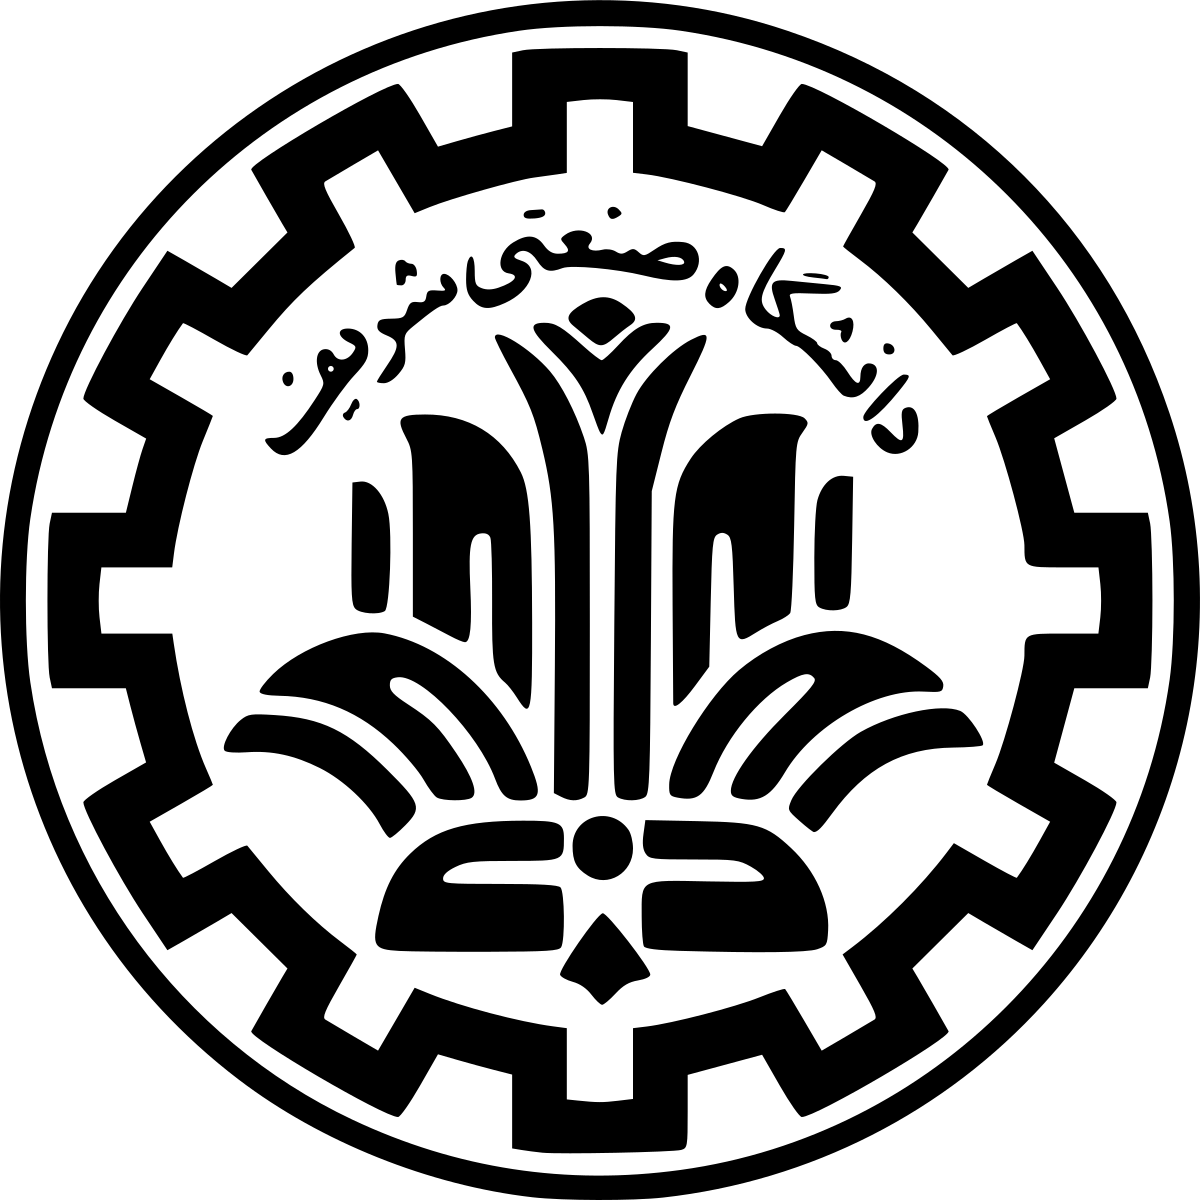
\includegraphics[width=4cm]{assets/logo-sharif.png} % آرم دانشگاه صنعتی شریف
			%			
			%			\vspace{1cm}
			%			
			%			{\huge \textbf{دانشگاه صنعتی شریف}}  
			%			
			%			\vspace{0.5cm}
			%			
			%			{\Large دانشکده مهندسی برق}
			%			
			%			\vspace{1.5cm}
			%			
			%			{\Huge \textbf{گزارش پروژه پایانی}} 
			%			
			%			\vspace{0.5cm}
			%			
			%			{\Large درس بهینه‌سازی محدب ۲}
			%			
			%			\vspace{1.5cm}
			%			
			%			{\Huge \textbf{یادگیری گراف با استفاده از همواری}}
			%			
			%			\vspace{1.5cm}
			%			
			%			\textbf{\Large استاد درس:}  
			%			
			%			\vspace{0.5cm}
			%			
			%			{\Large دکتر حامد شاه‌منصوری}
			%			
			%			\vspace{1.5cm}
			%			
			%			\textbf{\Large تهیه‌کنندگان:}  
			%			
			%			\vspace{0.5cm}
			%			
			%			{\Large محمد رضیئی فیجانی، علی مجلسی}
			%			
			%			\vfill
			%			
			%			{\Large \today}
			%			
			%		\end{center}
		%	\end{titlepage}
	
	\maketitle
	
	\section*{چکیده}
	\begin{strip}
		در کنار سیگنال های مرسوم که در زمان و یا فضا تعریف می‌شوند، دسته های جدیدی از سیگنال وجود دارند که به طور ذاتی بر روی گراف تعریف شده‌اند. یک مثل معروف تعاملات افراد در شبکه های اجتماعی است. تعریف سیگنال بر روی گراف امکان استفاده از ابزار های پردازش سیگنال گرافی مانند فیلتر کردن و تبدیل فوریه گرفتن را ممکن می‌کند. اولین قدم برای این کار ساخت گرافی از روی سیگنال‌های موجود است. که به آن یادگیری گراف اطلاق می‌شود. یکی از روش های تعیین این گراف استفاده از فاصله بین راس ها است به این صورت که اگر این فاصله از مقدار معینی کمتر بود بین دو راس، یال وجود داشته باشد. در این مقاله، یک روش تعیین گراف از روی سیگنال با به کارگیری خصوصیت همواری معرفی شده‌است که با بهره گیری از 
		\lr{Approximate Nearest Neighbors}
		پیچیدگی را به
		$nlog(n)D$
		کاهش داده است، که در آن n تعداد راس های گراف است و D ابعاد سیگنال روی گراف است. همچنین با استفاده از این الگوریتم می توان میانگین درجه راس ها را به مقدار دلخواه تعیین کرد.
	\end{strip}
	
	
	
	\section{مقدمه}
	در حوزه‌هایی که داده‌ها ساختار مشخصی ندارند، استفاده از گراف‌ها بسیار مفید است. برای مثال، سیگنال‌های زمانی دارای ساختاری هستند که ترتیب داده‌ها توسط بُعد زمان تعیین می‌شود، یا تصاویر که سیگنال‌های مکانی با ترتیب و مجاورت پیکسل‌ها مشخص می‌شوند. اما داده‌هایی نیز وجود دارند که ساختار مشخصی ندارند، مانند داده‌های سنسورهایی که دمای نقاط مختلف یک شهر را اندازه‌گیری می‌کنند و به‌صورت نامنظم در سطح شهر پراکنده‌اند، یا داده‌هایی با ساختار گراف‌مانند، مانند تعاملات کاربران در شبکه‌های اجتماعی نظیر اینستاگرام، جایی که سیگنال علاقه‌مندی هر کاربر می‌تواند در سیستم‌های توصیه‌گر استفاده شود.
	
	به همین دلیل، حوزه‌های جدیدی در پردازش سیگنال و شبکه‌های عصبی به نام 
	\textit{پردازش سیگنال گرافی}\LTRfootnote{Graph Signal Processing}(\lr{GSP})\cite{GSP}
	و
	\textit{شبکه‌های عصبی گراف}\LTRfootnote{Graph Neural Networks}(\lr{GNN})\cite{GNN}
	به وجود آمده‌اند.
	برای استفاده از روش‌های پردازش سیگنال روی گراف و شبکه‌های عصبی گراف ، ابتدا نیاز به یک ساختار گراف داریم که داده‌ها روی آن تعریف شوند. در بسیاری از موارد، داده‌های ما به‌صورت طبیعی دارای ساختار گرافی نیستند و باید این ساختار را از روی داده‌ها استخراج کنیم؛ فرآیندی که به آن 
	\textit{یادگیری گراف}\LTRfootnote{Graph Learning}
	گفته می‌شود.
	
	
	
	
	
	
	در یادگیری گراف، یکی از معیارهای کلیدی برای یافتن ساختار مناسب، هموار بودن داده‌ها روی گراف است. این معیار بیان می‌کند که در یک گراف بهینه، گره‌های متصل باید مقادیر مشابهی داشته باشند؛ به عبارت دیگر، داده‌ها نباید تغییرات ناگهانی در یال‌های گراف نشان دهند. برای مدل‌سازی این خاصیت، از انرژی دیریشله استفاده می‌شود که نشان‌دهنده‌ی میزان تغییرات داده‌ها روی گراف است. این انرژی بر اساس عملگر لاپلاسین گراف تعریف می‌شود:
	\begin{equation}
		\|\nabla_G \bm{X}\|_F^2 = \text{tr} (\bm{X}^\top \bm{L} \bm{X})
	\end{equation}
	
	در این رابطه، \( \nabla_G \bm{X} \) گرادیان گرافی داده‌های \( \bm{X} \) را نشان می‌دهد و \( \bm{L} \) ماتریس لاپلاسین گراف است که از رابطه‌ی زیر محاسبه می‌شود:
	
	\begin{equation}\label{eq:defL}
		\bm{L} = \bm{D} - \bm{W}
	\end{equation}
	
	که در آن \( \bm{D} \) ماتریس درجه است که مقدار مجموع وزن‌های یال‌های هر گره را در قطر خود دارد و \( \bm{W} \) ماتریس وزن‌های گراف است که ارتباط بین گره‌ها را نشان می‌دهد.
	\begin{equation}\label{eq:defD}
		\bm{D} = \operatorname{diag}(\bm{W}\mathds{1})
	\end{equation}
	
	انرژی دیریشله را می‌توان به‌صورت مجموع وزن‌دار اختلاف بین مقادیر گره‌ها نیز نوشت:
	\begin{equation}
		\frac{1}{2} \sum_{i,j} w_{ij} \|\bm{x}_i - \bm{x}_j\|_2^2
	\end{equation}
	
	این رابطه بیان می‌کند که مجموع اختلافات بین مقادیر گره‌های متصل، به وزن یال‌ها بستگی دارد. مقدار \( w_{ij} \) هرچه بیشتر باشد، یعنی ارتباط بین دو گره قوی‌تر است و در نتیجه اختلاف بین مقدار داده‌های آن دو گره باید کمتر باشد. برای نمایش دقیق‌تر این ارتباط، می‌توان از تعریف فاصله \( z_{ij} \) استفاده کرد:
	\begin{equation}
		z_{ij} = \|\bm{x}_i - \bm{x}_j\|^2
	\end{equation}
	
	در اینجا \( \bm{Z} \) ماتریس فاصله بین داده‌های متناظر با گره‌ها است. به این ترتیب، تابع بهینه‌سازی به‌صورت فشرده‌تر نوشته می‌شود:
	\begin{equation}
		\frac{1}{2} \| \bm{W} \circ \bm{Z} \|_{1,1}
	\end{equation}
	
	که در آن \( \circ \) عملگر ضرب هادامارد (عنصری) بین دو ماتریس است. این تابع نشان می‌دهد که یادگیری گراف بر مبنای هموار بودن داده‌ها، به یافتن ماتریس وزن‌های \( \bm{W} \) بستگی دارد که هموارترین تغییرات را در داده‌ها تضمین کند.
	
	برای یادگیری گراف با استفاده از معیار همواری، رویکردهای مختلفی پیشنهاد شده‌اند که هر کدام قیود متفاوتی بر روی ماتریس وزن‌های \( \bm{W} \) یا لاپلاسین \( \bm{L} \) اعمال می‌کنند. یکی از ساده‌ترین روش‌ها برای یادگیری گراف، کمینه‌سازی انرژی دیریشله \( \text{tr}(\|\bm{L} \bm{X}\|^2_F) \) تحت قیودی بر روی ماتریس وزن‌ها است.
	در روش \cite{Daitch2009}، این قیود شامل محدودیت \( \bm{W} \mathds{1} \geq \mathds{1} \) است که اطمینان می‌دهد هر گره حداقل مقدار مشخصی از اتصال را حفظ کند. 
	\begin{equation}
		\begin{array}{cl}
			\minimize{\bm{W}\in\mathcal{W}_m} & \text{tr}(\|\bm{L} \bm{X}\|^2_F) \\
			\text{\lr{subject to:}} & \bm{W} \mathds{1} \ge \mathds{1} \\
			& \eqref{eq:defD}, \eqref{eq:defL}
		\end{array}
	\end{equation}
	
	همچنین در نسخه دیگری از این روش، محدودیت \( \mathds{1}^\top \max(0, \bm{W} \mathds{1})^2 \leq \alpha n \) اعمال شده که میزان یال‌های اضافه را کنترل می‌کند. 
	\begin{equation}
		\begin{array}{cl}
			\minimize{\bm{W}\in\mathcal{W}_m} & \text{tr}(\|\bm{L} \bm{X}\|^2_F) \\
			\text{\lr{subject to:}} & \mathds{1}^\top \max(0, \bm{W} \mathds{1})^2 \leq \alpha n  \\
			& \eqref{eq:defD}, \eqref{eq:defL}
		\end{array}
	\end{equation}
	این قیود برای جلوگیری از یادگیری گراف‌های بیش‌ازحد متراکم و نامناسب طراحی شده‌اند. همچنین 
	$\mathcal{W}_m$
	مجموعه ماتریس های متقارن را نشان می‌دهد یعنی:
	\begin{equation}
		\mathcal{W}_m = \big\{\bm{W} | \bm{W} = \bm{W}^\top, \bm{W} \in \mathds{R}_+^{n\times n}\big\}
	\end{equation}
	
	مدل \cite{Lake2010DiscoveringSB} تابع هدف را گسترش داده و از یک ترم لگاریتمی روی دترمینان لاپلاسین به همراه یک منظم‌کننده‌ی \( \ell_1 \) روی ماتریس وزن‌ها استفاده می‌کند:
	\begin{equation}
		\minimize{\bm{W}} \text{tr} (\bm{X}^\top \bm{L} \bm{X}) - \log | \bm{L} + \alpha \bm{I} | + \beta \| \bm{W} \|_{1,1}
	\end{equation}
	
	ترم \( \log | \bm{L} + \alpha \bm{I} | \) از تکین شدن \( \bm{L} \) جلوگیری می‌کند و منظم‌کننده \( \ell_1 \) باعث می‌شود که بسیاری از درایه‌های \( \bm{W} \) صفر شوند، که منجر به یادگیری یک گراف تنک می‌شود.
	
	در روش‌های
	\cite{Hu2015,Dong2016}
	علاوه بر انرژی دیریشله، یک ترم اضافی نرم فروبنیوس برای کنترل مقدار \( \bm{L} \) اضافه شده است:
	
	\begin{equation}
		\begin{array}{cl}
			\minimize{\bm{L}} & \text{tr} (\bm{X}^\top \bm{L} \bm{X}) + \alpha \|\bm{L}\|_F^2 \\
			\text{\lr{subject to}} & \text{tr}(\bm{L}) = n
		\end{array}
	\end{equation}
	
	وجود \( \|\bm{L}\|_F^2 \) در تابع هدف به جلوگیری از مقدارهای بیش‌ازحد بزرگ در ماتریس لاپلاسین کمک می‌کند و شرط \( \text{tr}(\bm{L}) = n \) مقیاس گراف را کنترل می‌کند تا بیش از حد کوچک یا پراکنده نشود.
	
	مدل 
	\cite{Kalofolias2016}
	با اضافه کردن یک ترم لگاریتمی روی مجموع وزن‌ها و یک منظم‌کننده‌ی نرم فروبنیوس برای کنترل پیچیدگی گراف، یک روش جامع‌تر برای یادگیری گراف ارائه می‌دهد:
	
	\begin{equation}
		\minimize{\bm{W}\in\mathcal{W}_m} \text{tr} (\bm{X}^\top \bm{L} \bm{X}) - \alpha \mathds{1}^\top \log (\bm{W} \mathds{1}) + \frac{\beta}{2} \|\bm{W}\|_F^2
	\end{equation}
	
	ترم \( \mathds{1}^\top \log (\bm{W} \mathds{1}) \) باعث می‌شود که وزن‌های گراف به شکلی کنترل‌شده توزیع شوند و از تشکیل یال‌های بیش از حد ضعیف یا بسیار قوی جلوگیری شود، در حالی که ترم \( \|\bm{W}\|_F^2 \) از مقدارهای بیش‌ازحد بزرگ در وزن‌های یال‌ها جلوگیری می‌کند. این روش یک رویکرد بهینه برای یادگیری گراف‌های هموار ارائه می‌دهد که می‌تواند در کاربردهای مختلفی از جمله تحلیل شبکه‌های اجتماعی، پردازش سیگنال‌های گرافی و مدل‌سازی داده‌های غیرساختاریافته مورد استفاده قرار گیرد.
	
	هر یک از این روش‌ها، به طور خاص در تنظیم مقادیر یال‌ها و بهینه‌سازی لاپلاسین گراف مؤثر هستند و بسته به ویژگی‌های داده و نیازمندی‌های خاص یک مسئله، انتخاب مناسبی از میان این مدل‌ها می‌تواند صورت گیرد. مدل‌هایی که شامل قیود حداقلی برای درجه گره‌ها هستند، برای کاربردهایی مناسب‌اند که در آن‌ها اتصال حداقلی بین گره‌ها ضروری است. از سوی دیگر، روش‌هایی که از منظم‌کننده‌های \(\ell_1\) یا \(\ell_2\) استفاده می‌کنند، در یادگیری گراف‌های تنک کارایی بالاتری دارند، زیرا از ایجاد ارتباطات غیرضروری بین گره‌ها جلوگیری می‌کنند. همچنین، مدل‌هایی که از تابع لگاریتمی روی دترمینان لاپلاسین بهره می‌برند، تضمین می‌کنند که ساختار گراف دچار مشکلات عددی ناشی از تکین شدن ماتریس لاپلاسین نشود.
	
	در نهایت، تعادل میان پیچیدگی ساختاری گراف و میزان همواری داده‌ها، به عنوان یک مسئله‌ی بهینه‌سازی در یادگیری گراف مطرح می‌شود. مدل‌های مختلف ارائه‌شده نشان می‌دهند که می‌توان با انتخاب مناسب تابع هدف و قیود مربوطه، ساختار گرافی مطلوبی را یاد گرفت که ویژگی‌های ذاتی داده‌ها را به خوبی بازتاب دهد. این حوزه از تحقیق همچنان در حال پیشرفت است و روش‌های جدیدتر با در نظر گرفتن قیود فیزیکی، توپولوژیکی و داده‌محور، در حال توسعه هستند تا فرآیند یادگیری گراف را بهینه‌تر و کاربردی‌تر کنند.
	
	
	
	\section{صورت مسئله}
	
	در این گزارش، فرآیند یادگیری گراف با تابع هزینه سه جمله ای شامل همواری گراف و 
	\textit{سد لگاریتمی}\LTRfootnote{logarithmic barrier}
	 که باعث می شود به هر راس حداق یک یال وصل باشد و نرم فروبنیوس که ترم رگیولاریزیشن آن است که باعث می‌شود نه وزن ها نامتعادل 
	\cite{Kalofolias2016} 
	مورد بررسی قرار گرفته است. هدف این روش، یادگیری یک گراف از سیگنال‌های هموار
	\LTRfootnote{Smooth Signals} 
	است به‌طوری‌که ساختار گراف به‌طور بهینه با داده‌ها سازگار باشد. تابع هزینه نهایی در معادله 
	\ref{eq:opt1}
	نشان داده شده است.
	
	هدف پیدا کردن جواب مسئله بهینه سازی
	\ref{eq:opt1}
	است. این مسئله یک مسئله بهینه سازی محدب است. 
	\begin{equation}\label{eq:opt1}
		\begin{array}{cl}
			\arg \minimize{\mathbf{W_{n \times n}}} &\sum_{i,j} \left\| \mathbf{x}(i) - \mathbf{x}(j) \right\|^2 w_{ij} \\ &\quad - \alpha \sum_{i=1}^{n} \log \left( \sum_{k=1}^{n} w_{ik} \right) + \frac{\beta}{2} \left\| \mathbf{W} \right\|_F^2 \\
			\text{\lr{subject to:}} & w_{ij} \geq 0
		\end{array}
	\end{equation}
	\section{حل مسئله‌ی بهینه سازی} \label{sec:optsol}
	
	برای حل این مسئله از الگوریتم ADMM استفاده شده است. زمان اجرای این الگوریتم به دلیل بهینه سازی جداگانه هر کدام از متغییر ها، نسبت به تعداد متغیر ها به صورت خطی افزایش می یابد به همین دلیل این الگوریتم انتخاب شده است.
	
	برای نوشتن مسئله به فرم جدایی پذیر و حل آن با ADMM تنها جزء جدایی ناپذیر
	مسئله را که به‌صورت
	$
	\sum_{l=1}^{n} \ln \left( \sum_{j=1}^{n} w_{ij} \right)
	$
	است، با تعریف متغیر کمکی 	$S_i := \sum_{j=1}^{n} w_{ij}$	به قید تساوی تبدیل می‌شود.
	
	
	
	\begin{equation}\label{eq:opt2}
		\begin{array}{cl}
			\arg \minimize{\mathbf{W_{n \times n}}}&\sum_{i,j} \left\| \mathbf{x}_i - \mathbf{x}_j \right\|^2 w_{ij}
			\\&\qquad- \alpha \sum_{i=1}^{n} \log \left( d_i \right) + \frac{\beta}{2} \left\| \mathbf{W} \right\|_F^2 \\
			\text{\lr{subject to:}} &d_i = \sum_{j=1}^{n} w_{ij}, \quad w_{ij} > 0
		\end{array}
	\end{equation}
	
	اکنون مسئله به مسئله بهینه‌سازی یک تابع محدب با قید تساوی تبدیل شده است.
	
	قید نامساوی $w_{ij} \geq 0$ را می‌توان با تصویر کردن ضرایب \( w_{ij} \)
	در هر مرحله تکرار با رابطه $w_{ij} = \max(w_{ij}, 0)$ برآورده کرد.
	
	در نهایت با توجه به الگوریتم ADMM می‌توان بهینه‌سازی را با الگوریتم زیر انجام داد:
	
	\begin{equation}\label{eq:opt3}
		\begin{array}{cl}
			L_{\rho} (W, s, \nu) = &\sum_{i,j} w_{ij} \left\| x_i - x_j \right\|^2 - \alpha \sum_{l=1}^{n} \ln (s_i) \\
			&\qquad+ \frac{\beta}{2} \sum_{i,j} (w_{ij})^2 \\
			&\qquad+ \sum_{i=1}^{N} \nu_i \big( s_i - \sum_{j=1}^{n} w_{ij} \big)\\
			&\qquad+ \frac{\rho}{2} \sum_{i=1}^{n} \big( s_i - \sum_{j=1}^{N} w_{ij} \big)^2
		\end{array}
	\end{equation}
	
	\begin{equation}\label{eq:admm_alg}
		\begin{aligned}
			&w_{ij}^{k+1} = \arg\min L_{\rho} (W, S^k, V^k)\\
			&s_{ij}^{k+1} = \arg\min L_{\rho} (W^k, s, V^k)\\
			&\nu^{k+1} = \nu^k + \rho \big( s_i - \sum_{j=1}^{n} W_{ij} \big)
		\end{aligned}
	\end{equation}
	مقادیر argmin در معادله \ref{eq:admm_alg} با مشتق گیری به صورت تحلیلی و برابر صفر گذاشتن مشتق می‌توان پیدا کرد.
	\begin{equation}\label{eq:iter}
		\begin{array}{cl}
			&w_{ij}^{k+1} = \max \big( \frac{1}{\beta + \rho} \big( \nu_i^k + \rho s_i + \sum_{j=1}^{N} w_{ij}^k - \|x_i^k - x_j^k\|^2 \big), 0 \big) \\
			&s_i^{k+1} = \max \Big( \frac{1}{2\rho} \big( -\big( \nu_i^k - \rho \sum_{j=1}^{N} w_{ij}^k \big) \\
			&\qquad\qquad\qquad\pm \sqrt{\big( \nu_i^k - \rho w_{ij}^k \big)^2 + 4\alpha \rho} \big), 0 \Big) \\
			&\nu_i^{k+1} = \nu_i^k + \rho \left( s_i - \sum_{j=1}^{N} w_{ij} \right)
		\end{array}
	\end{equation}
	در نهایت با چند بار تکرار معادله \ref{eq:iter} مقادیر $w_{ij}$ به مقدار بهینه همگرا خواهد شد. همچنین با استفاده از الگوریتم های
	\lr{Approximate Nearest Neighbor (ANN)}
	مولفه هایی از $w_{ij}$ که فاصله $x_i$ و $x_j$ از یکدیگر زیاد باشد، صفر در نظر گرفته می‌شود و زمان محاسبه حاصل جمع های معاله \ref{eq:iter} از
	\lr{O(n)}
	به
	\lr{O(k)}
	که k درجه راس های گراف است کاهش می یابد.
	
	\section{تعیین مقادیر پارامتر های $\alpha$ و $\beta$}
	در فرآیند یادگیری گراف، انتخاب پارامترهای مناسب تأثیر مستقیمی بر ساختار و تراکم گراف دارد. دو پارامتر کلیدی \( \alpha \) و \( \beta \) تنظیم‌کننده‌ی رفتار بهینه‌سازی هستند که بر مقیاس‌بندی وزن‌های یال‌ها و میزان تراکم گراف اثر می‌گذارند. تابع بهینه‌سازی پایه‌ای برای یافتن ماتریس وزن‌های \( \bm{W}^* \) به‌صورت زیر تعریف می‌شود:
	
	\[
	\bm{W}^*(\bm{Z}, \alpha, \beta) = \arg \min_{\bm{W} \in \mathcal{W}_m} \|\bm{W} \circ \bm{Z}\|_{1,1} - \alpha \mathds{1}^\top \log(\bm{W} \mathds{1}) + \frac{\beta}{2} \|\bm{W}\|_F^2
	\]
	
	در این تابع هزینه، ترم \( \|\bm{W} \circ \bm{Z}\|_{1,1} \) فاصله‌ی بین گره‌ها را در نظر می‌گیرد و همواری داده‌ها را حفظ می‌کند. ترم \( \alpha \mathds{1}^\top \log(\bm{W} \mathds{1}) \) توزیع یال‌ها و میزان درجه‌ی هر گره را کنترل می‌کند، در حالی که \( \frac{\beta}{2} \|\bm{W}\|_F^2 \) به‌عنوان یک منظم‌کننده‌ی فروبنیوس، مقدارهای بزرگ در وزن‌های یال‌ها را کاهش می‌دهد.
	
	برای ساده‌سازی این مسئله، یک ضریب مقیاس‌گذاری \( \delta \) تعریف می‌شود:
	
	\[
	\delta = \sqrt{\frac{\alpha}{\beta}}
	\]
	
	که اجازه می‌دهد تابع هزینه به فرم ساده‌تری تغییر یابد:
	\begin{align}
		\bm{W}^*(\bm{Z}, \alpha, \beta) = \delta \arg \minimize{\bm{W} \in \mathcal{W}_m} \|\bm{W} \circ \bm{Z}\|_{1,1} 
		- \mathds{1}^\top \log(\bm{W} \mathds{1}) + \frac{1}{2} \|\bm{W}\|_F^2
	\end{align}
	
	ضریب \( \delta \) تنها مقیاس مقدارهای وزن یال‌ها را تغییر می‌دهد و مستقیماً بر میزان تراکم گراف تأثیر نمی‌گذارد. در عوض، عامل تعیین‌کننده‌ی میزان یال‌های گراف، پارامتر \( \theta \) است که به‌صورت زیر تعریف می‌شود:
	
	\[
	\theta = \sqrt{\frac{1}{\alpha \beta}}
	\]
	
	و اجازه می‌دهد تابع هزینه به شکل نهایی زیر بازنویسی شود:
	
	\[
	\bm{W}^*(\bm{Z}, \alpha, \beta) = \delta \bm{W}^*(\theta \bm{Z}, 1, 1)
	\]
	
	این رابطه نشان می‌دهد که مقدار \( \theta \) مستقیماً تعداد یال‌های گراف را تنظیم می‌کند، در حالی که \( \delta \) صرفاً بر مقیاس وزن‌های یال تأثیر می‌گذارد. بنابراین، می‌توان مقدار مطلوبی از یال‌ها را با انتخاب مناسب \( \theta \) تعیین کرد، بدون نیاز به جستجوی گسترده در فضای پارامترها.
	
	برای تحلیل دقیق‌تر نقش \( \theta \)، مسئله‌ی بهینه‌سازی را می‌توان برای یک گره منفرد ساده کرد. در این حالت، تنها یک ستون از ماتریس وزن‌ها در نظر گرفته می‌شود و تقارن وزن‌ها نادیده گرفته می‌شود، که منجر به مسئله‌ی زیر می‌شود:
	
	\[
	\minimize{\bm{w} \geq 0} \theta \bm{w}^\top \bm{z} - \log(\bm{w}^\top \mathds{1}) + \frac{1}{2} \|\bm{w}\|_2^2
	\]
	
	در این تابع، ترم \( \theta \bm{w}^\top \bm{z} \) فاصله‌های بین گره‌ها را در نظر می‌گیرد که توسط \( \theta \) مقیاس‌بندی می‌شود. ترم \( \log(\bm{w}^\top \mathds{1}) \) توزیع یال‌ها را کنترل می‌کند و مجموع وزن‌های هر گره را تنظیم می‌کند، در حالی که ترم \( \frac{1}{2} \|\bm{w}\|_2^2 \) مقدارهای بیش‌ازحد بزرگ را منظم می‌کند. این مسئله نشان می‌دهد که \( \theta \) مستقیماً بر میزان یال‌های موجود در گراف اثر دارد و می‌توان مقدار مناسب آن را برای تنظیم پراکندگی گراف انتخاب کرد.
	
	تحلیل دقیق نشان می‌دهد که اگر مقدار \( \theta \) در بازه‌ی مشخصی قرار گیرد، تعداد دقیق یال‌های غیرصفر برای هر گره برابر با مقدار \( k \) خواهد شد:
	
	\begin{equation}
		\left( \frac{1}{\sqrt{k z_k^2 - b_k z_{k+1}}}, \frac{1}{\sqrt{k z_k^2 - b_k z_k}} \right)
	\end{equation}
	
	این رابطه نشان می‌دهد که تنظیم مقدار \( \theta \) به ما امکان می‌دهد که تعداد یال‌های غیرصفر در هر گره را کنترل کنیم. این ویژگی به‌خصوص در یادگیری گراف‌های تنک بسیار مفید است، زیرا اجازه می‌دهد که ساختار گراف را با توجه به نیاز مسئله تنظیم کرده و از ایجاد یال‌های غیرضروری جلوگیری کنیم.
	
	در مقیاس کل گراف، مقدار \( \theta \) به گونه‌ای انتخاب می‌شود که میانگین تعداد یال‌های هر گره برابر با مقدار دلخواه باشد. در این حالت، مقدار مناسب \( \theta \) باید به گونه‌ای تنظیم شود که تعداد یال‌های گره‌ها در سراسر گراف به‌طور میانگین برابر مقدار هدف باشد. این مقدار را می‌توان از رابطه‌ی تحلیلی بین \( \theta \) و میانگین تعداد یال‌های هر گره استخراج کرد:
	
	\[
	\mathbb{E}[d] \approx k
	\]
	
	که در آن \( \mathbb{E}[d] \) مقدار مورد انتظار برای تعداد یال‌های هر گره است. مقدار مناسب \( \theta \) را می‌توان از طریق رابطه‌ای که میانگین درجه‌ی گره‌ها را کنترل می‌کند، تعیین کرد. نتایج تجربی نشان داده‌اند که مقدار اندازه‌گیری‌شده‌ی تراکم گره‌ها با حدود نظری تخمین‌زده‌شده برای \( \theta \) مطابقت دارد. این روش امکان یادگیری گراف با تعداد یال‌های کنترل‌شده را بدون نیاز به آزمایش‌های متعدد فراهم می‌کند و رویکردی تحلیلی و کارآمدتر نسبت به روش‌های کلاسیک که نیاز به تنظیم دستی دارند، ارائه می‌دهد.
	
	
	\section{شبیه سازی}
	
	
	\subsection{با داده های مصنوعی}
	
	\subsection{با داده های واقعی}
	
	\begin{figure}[H]
		\centering
		\begin{adjustbox}{scale=.9}
			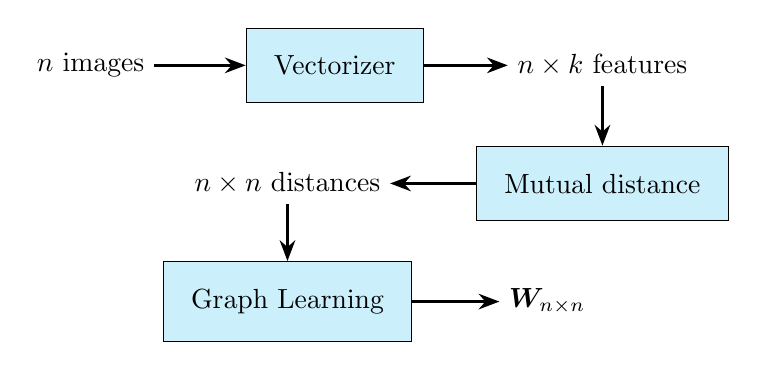
\begin{tikzpicture}[every node/.style={}]
				\node (image) at (0,0) {$n$ images};
				\node[fill=cyan!20,draw=black,radius=5pt,inner sep=10pt] (vectorizer) at (3.1,0) {Vectorizer};
				\node (features) at (6.5,0) {$n\times k$ features};
				\node[fill=cyan!20,draw=black,radius=5pt,inner sep=10pt] (distance) at (6.5,-1.5) {Mutual distance};
				\node (zdist) at (2.5,-1.5) {$n\times n$ distances};
				\node[fill=cyan!20,draw=black,radius=5pt,inner sep=10pt] (graphlearning) at (2.5,-3) {Graph Learning};
				\node (weights) at (5.8,-3) {$\bm{W}_{n\times n}$};
				
				\draw[-Stealth,line width=1] (image) -- (vectorizer);
				\draw[-Stealth,line width=1] (vectorizer) -- (features);
				\draw[-Stealth,line width=1] (features) -- (distance);
				\draw[-Stealth,line width=1] (distance) -- (zdist);
				\draw[-Stealth,line width=1] (zdist) -- (graphlearning);
				\draw[-Stealth,line width=1] (graphlearning) -- (weights);
			\end{tikzpicture}
		\end{adjustbox}
		\caption{
		فلوچارت الگوریتم برای داده های 
		\lr{IMAGENET}
		}
	\end{figure}
	
	

	
	\section{نتایج}
	برای ارزیابی مدل، یک شبکه $16\times16$  مطابق شکل \ref{fig:graph-initial-1}  تولید شده است. سپس به مختصات (x,y) این شبکه، نویز تصادفی اضافه شده است تا کمی نقاط از جای اصلی خود جا به جا شوند. گراف متناظر با این نقاط با ماکزیمم درجه راس 4
	\lr{(k=4)}
	بدست آمده است. گراف نهایی در شکل
	\ref{fig:graph-final-1}
	نشان داده شده است.
	\begin{figure}[H]
		\centering
		\adjincludegraphics[width=0.9\linewidth,trim={{.12\width} {.12\height} {.12\width} {.1\height}} ,clip]{codes/results/graph-initial.pdf}
		\caption{ساختار گراف اولیه.}
		\label{fig:graph-initial-1}
	\end{figure}
	
	\begin{figure}[H]
		\centering
		\adjincludegraphics[width=0.9\linewidth,trim={{.12\width} {.12\height} {.12\width} {.1\height}} ,clip]{codes/results/graph-final.pdf}
		\caption{ساختار نهایی گراف.}
		\label{fig:graph-final-1}
	\end{figure}
	همچنین برای نشان دادن تنک بودن
	\LTRfootnote{Sparsity}
	گراف بدست آمده، ماتریس ضرایب در شکل
	\ref{fig:graph-learned-k4-1}
	نمایش داده شده است.
	
	\begin{figure}[H]
		\centering
		\includegraphics[width=0.7\linewidth]{codes/results/graph-learned-k4.pdf}
		\caption{
			ماتریس وزن های گراف یادگرفته‌شده با \( k = 4 \) یال در هر گره به‌طور متوسط.
		}
		\label{fig:graph-learned-k4-1}
	\end{figure}
	
	\section{نتیجه گیری}
	در این گزارش نحوه پیدا کردن گراف مناسب روی مجموعه از سیگنال ها بررسی شد. این مسئله منجر به بهینه سازی تابع هزینه معادله
	\ref{eq:opt1}
	شد. که یک مسئله بهینه سازی محدب است. در نهایت الگوریتمی برای حل مسئله با روش ADMM ارائه شد. برای کاهش مرتبه پیچیدگی این الگوریتم با استفاده از Approximation Nearest Neighbor مرتبه پیچیدگی الگوریتم به
	\lr{O(kn)}
	است که k متوسط درجه راس های گراف و د تعداد رئوس گراف است. همچنین در این گزارش روشی برای تخمین پارامتر های $\alpha$ و $\beta$ برای دستیابی به میانگین درجه رئوس k پیشنهاد شده است. \\
	
	بخش های مقدمه، صورت مسئله، تعیین مقادیر پارمتر های 
	$\alpha$ و $\beta$
	، شبیه‌سازی و پیوست ها توسط آقای رضیئی نوشته شده است و بخش های چکیده، حل مسئله بهینه سازی و نتیجه گیری توسط آقای مجلسی نوشته شده است.\\
	
	این مسئله در MATLAB پیاده سازی شده است که جرئیات این پیاده سازی در  بخش پیوست ها
	\ref{sec:append}
	آمده است. \\
	
	جزئیات حل مسئله با روش ADMM که در بخش
	\ref{sec:optsol}
	آمده است و روابط نهایی 
	\ref{eq:iter}
	جزء نوآوری های این گزارش است و در مقالات ارجاع داده شده وجود ندارد.
	

	
	
	\bibliographystyle{plainnat-fa}
	\bibliography{assets/references}
	\nocite{*}
	
	
	
	\clearpage
	
	\section*{پیوست ها}\label{sec:append}
	\appendix
	
	\section{فرآیند یادگیری گراف}
	
	ابتدا یک گراف اولیه به‌صورت شبکه‌ی دوبعدی با نویز تصادفی ایجاد می‌شود. مختصات گره‌ها شامل مقداری نویز است تا تنوع داده‌ها افزایش یابد.
	
	\begin{latin}
		\lstinputlisting[firstline=4,lastline=10]{codes/simple.m}
	\end{latin}
	
	\begin{figure}[H]
		\centering
		\includegraphics[width=0.7\linewidth]{codes/results/graph-initial.pdf}
		\caption{ساختار گراف اولیه.}
		\label{fig:graph-initial}
	\end{figure}
	
	\subsection{ماتریس فواصل جفتی}
	برای یادگیری گراف، ابتدا ماتریس فواصل جفتی \( Z \) محاسبه می‌شود. این ماتریس به‌صورت زیر تعریف می‌شود:
	
	\[
	Z_{ij} = \|\mathbf{x}_i - \mathbf{x}_j\|^2
	\]
	
	که در آن \( \mathbf{x}_i \) و \( \mathbf{x}_j \) مختصات گره‌های \( i \) و \( j \) هستند.
	
	\begin{latin}
		\lstinputlisting[firstline=13,lastline=17]{codes/simple.m}
	\end{latin}
	
	
	\begin{figure}[H]
		\centering
		\includegraphics[width=0.7\linewidth]{codes/results/pairwise-distances.pdf}
		\caption{ماتریس فواصل جفتی \( Z \).}
		\label{fig:pairwise-distances}
	\end{figure}
	

	در این مرحله، با استفاده از روش \cite{Kalofolias2016} و با تنظیم پارامترهای \( a = 1 \) و \( b = 1 \)، ماتریس وزن‌های گراف \( W \) یاد گرفته می‌شود. تابع هدف به‌صورت زیر است:
	
	\[
	\min_{\bm{W}} \sum_{i,j} z_{ij} w_{ij} + a \sum_{i,j} {w}_{ij} \log {w}_{ij} + b \|\bm{W}\|_F^2
	\]
	
	که در آن
	\( \|\bm{W}\|_F \)
	نرم فروبنیوس ماتریس \( W \) است.
	
	\begin{latin}
		\lstinputlisting[firstline=20,lastline=26]{codes/simple.m}
	\end{latin}
	
	\begin{figure}[H]
		\centering
		\includegraphics[width=0.7\linewidth]{codes/results/graph-learned-ab1.pdf}
		\caption{گراف یادگرفته‌شده با \( a = 1 \) و \( b = 1 \).}
		\label{fig:graph-learned-ab1}
	\end{figure}
	
	برای کنترل میزان پراکندگی گراف، می‌توان پارامتر \( \theta \) را به‌گونه‌ای تنظیم کرد که هر گره به‌طور متوسط دارای \( k \) یال باشد. 
	
	\begin{latin}
		\lstinputlisting[firstline=29,lastline=44]{codes/simple.m}
	\end{latin}
	
	
	\begin{figure}[H]
		\centering
		\includegraphics[width=0.7\linewidth]{codes/results/graph-learned-k4.pdf}
		\caption{گراف یادگرفته‌شده با \( k = 4 \) یال در هر گره به‌طور متوسط.}
		\label{fig:graph-learned-k4}
	\end{figure}
	
	\subsection{نمایش نهایی گراف}
	در نهایت، ساختار گراف یادگرفته‌شده به‌صورت بهینه و با کاهش اتصالات ضعیف نمایش داده می‌شود.
	
	\begin{latin}
		\lstinputlisting[firstline=47,lastline=49]{codes/simple.m}
	\end{latin}
	
	
	\begin{figure}[H]
		\centering
		\includegraphics[width=0.7\linewidth]{codes/results/graph-final.pdf}
		\caption{ساختار نهایی گراف.}
		\label{fig:graph-final}
	\end{figure}
	
	
	
	
	
\end{document}